\documentclass[tikz,border=3.14mm]{standalone}
\usepackage{pgfplots}
\pgfplotsset{compat=1.17}

\begin{document}
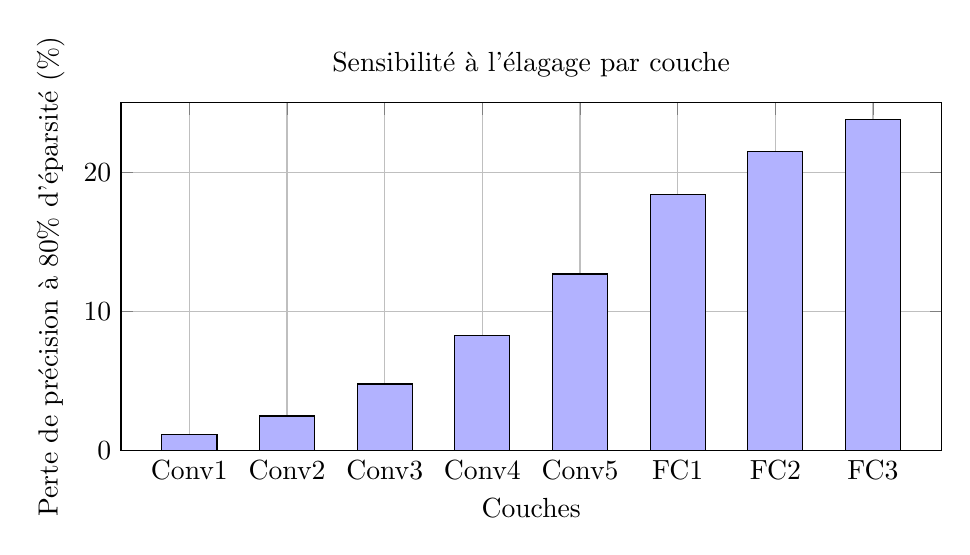
\begin{tikzpicture}
\begin{axis}[
    title={Sensibilité à l'élagage par couche},
    xlabel={Couches},
    ylabel={Perte de précision à 80\% d'éparsité (\%)},
    symbolic x coords={Conv1, Conv2, Conv3, Conv4, Conv5, FC1, FC2, FC3},
    xtick=data,
    ymin=0, ymax=25,
    grid=both,
    width=12cm,
    height=6cm,
    bar width=0.7cm
]

\addplot[ybar, fill=blue!30] coordinates {
    (Conv1, 1.2)
    (Conv2, 2.5)
    (Conv3, 4.8)
    (Conv4, 8.3)
    (Conv5, 12.7)
    (FC1, 18.4)
    (FC2, 21.5)
    (FC3, 23.8)
};

\end{axis}
\end{tikzpicture}
\end{document}